%Metroplolis Beamer Theme: https://github.com/matze/mtheme
\documentclass[aspectratio=169, 10pt]{beamer}

\usetheme{metropolis}
\usepackage{appendixnumberbeamer, lmodern, bookmark, kbordermatrix,fontawesome}
\usepackage{booktabs}
% \usepackage[sorting=none]{biblatex}
\usepackage[scale=2]{ccicons}

\usepackage{pgfplots}
\usepgfplotslibrary{dateplot}

\usepackage{xspace}
\newcommand{\themename}{\textbf{\textsc{metropolis}}\xspace}

\title{The emergence of geometric order \\ in proliferating metazoan epithelia.}
\subtitle{by Gibson \emph{et al}. \textit{Nature}, 2006 \\Computational Biology and Bioinformatics Seminar}
\date{\today}
\author{Philip Hartout}
\institute{ETH Zurich} 
% \titlegraphic{\hfill\includegraphics[height=1.5cm]{logo.pdf}}

\usepackage[style=british]{csquotes}

\def\signed #1{{\leavevmode\unskip\nobreak\hfil\penalty50\hskip1em
  \hbox{}\nobreak\hfill #1%
  \parfillskip=0pt \finalhyphendemerits=0 \endgraf}}

\newsavebox\mybox
\newenvironment{aquote}[1]
  {\savebox\mybox{#1}\begin{quote}\openautoquote\hspace*{-.7ex}}
  {\unskip\closeautoquote\vspace*{1mm}\signed{\usebox\mybox}\end{quote}}


\begin{document}

\maketitle

\begin{frame}{Table of contents}
  \setbeamertemplate{section in toc}[sections numbered]
  \tableofcontents[hideallsubsections]
\end{frame}

\section{Introduction}

\begin{frame}[fragile]{Motivation}

    \begin{aquote}{Gibson \emph{et al} \cite{gibson2006emergence}}
    The organisation of cells into epithelial sheets is an essential feature of animal design.
    \end{aquote}

\end{frame}

\begin{frame}[fragile]{Context}
    Predictable geometries arise when \textit{minimising surface energy} or \textit{maximising space filling} in biological and non-biological structures:
    \begin{columns}[T,onlytextwidth]
        \column{0.5\textwidth}
          Examples
          \begin{itemize}
            \item \textit{Drosophila Melanogaster}'s retinal cells \item Honeycombs \item Coins on tabletops
          \end{itemize}
    
        \column{0.5\textwidth}
            \begin{figure}
                \centering
                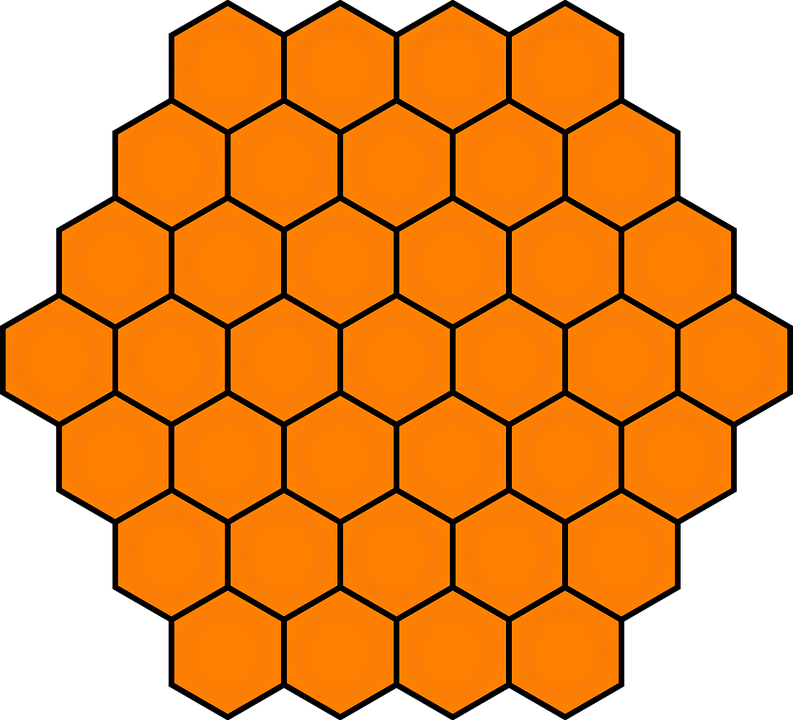
\includegraphics[width=.5\textwidth]{presentation/figures/honeycombs.png}
                \label{}
            \end{figure}
    \end{columns}
    \vspace{12pt}
    \onslide<2->How is the geometry of \emph{growing} epithelial cells organized and how can it be explained? 
\end{frame}

\begin{frame}[fragile]{Emergent behaviour}  
    Understanding emergent behaviours is required to model geometries of growing epithelial cells.
    \onslide<2->\begin{alertblock}{Emergent behaviour}
        \vspace{5pt}
        It is the behaviour of a system that can \emph{only} be explained by examination of a system's \textbf{parts} \emph{and} their \textbf{relationships}.
    \end{alertblock}
\end{frame}

\section{Model Assumptions}

\begin{frame}[fragile]{Post-mitotic relationship between two daughter cells}
  Stochastically marked cell lineages with GFP revealed stable post-mitotic patterns.     
  \begin{columns}[]
    \column{0.5\textwidth}  
    \begin{figure}[b]
      \centering
      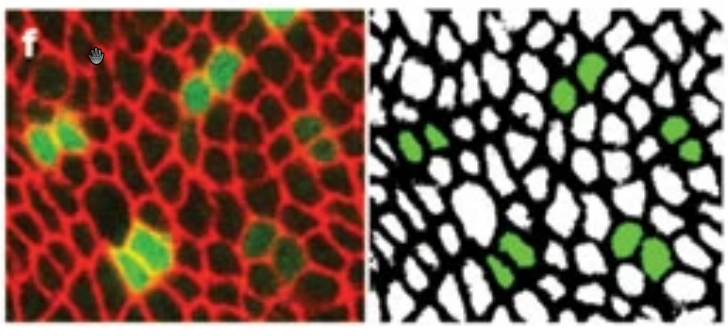
\includegraphics[width=\textwidth]{presentation/figures/daughter-cell-relationship.png}
      \caption{Daugher-cell relationship.}
      \label{}
    \end{figure}
    \column{0.5\textwidth}
        \begin{figure}[b]
            \centering
            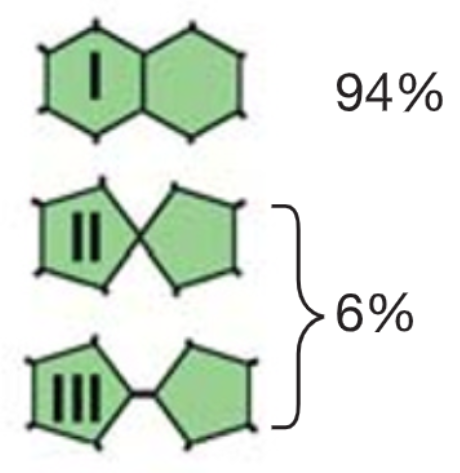
\includegraphics[width=.4\textwidth]{presentation/figures/post-mitotic-relationship.png}
            \caption{Observed post-mitotic relationship between daughter cells.}
            \label{}
    \end{figure}
  \end{columns}  
  \onslide<2->$\rightarrow$ required to model relationships between cells
\end{frame}

\begin{frame}[fragile]{Typical topology changes of a dividing cell}
  \begin{figure}[]
    \centering
    \caption{Topology changes during cell division}
    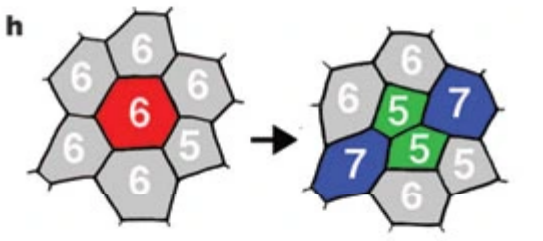
\includegraphics[width=.5\textwidth]{presentation/figures/topology_evolution.png} 
    \label{}
  \end{figure}
\end{frame}

\section{A Discrete Markov Model for Proliferating Epithelia}

\begin{frame}[fragile]{Markov models}
    A Markov chain is a discrete stochastic process with the Markov property:
    \begin{equation*}
      P(X_t|X_{t-1},\ldots,X_1)=P(X_t|X_{t-1})
    \end{equation*}
    where $X_t$ is the time-dependent r.v. describing the state of the system at time $t$. 
    
    It is determined by a probability transition matrix $P$ and an initial probability distribution. 

\end{frame}

\begin{frame}[fragile]{Applying a discrete Markov model to growing epithelkiia}
  \begin{columns}
    \column{\textwidth}
    \begin{table}
      \centering
      \scalebox{.9}{
      \begin{tabular}{lp{12.5cm}}
        $s$ & state of the cell as its number of sides, where $s>3$.\\  
        \onslide<2->$p_s$ & the relative frequency of $s$-sided cells in the population \\
        \onslide<3->$\mathbf{p}^{(t)}$ & the infinite row vector $\mathbf{p}^{(t)}=[p_4, p_5, p_6,\ldots ]$ state of the population at generation $t$.\\
        \onslide<4->$\mathbf{p}^{(t+1)}=\mathbf{p}^{(t)}PS$ & the state dynamics, where $P$ and $S$ are the probabilistic transition matrices.\\
        \onslide<5->$P_{ij}$ & the probability that an $i$ sided cell divides to produce a $j$-sided daughter cell.\\
        \onslide<6->$S_{ij}$ & the probability of an $i$-sided cell will gain sides from dividing neighbour cells divisions to become $j$-sided. \\
      \end{tabular}}
    \end{table}
  \end{columns}
\end{frame}

\begin{frame}[fragile]{Transition matrices}
  \begin{columns}[onlytextwidth]
    \column{0.5\textwidth}
    \renewcommand{\kbldelim}{(}% Left delimiter
    \renewcommand{\kbrdelim}{)}% Right delimiter
    \[
      P = \kbordermatrix{
        & 4 & 5 & 6 & 7 & 8 & 9 & \ldots\\
        4 & 1 &  &  &  & & &  \\
        5 & 1 & 1 & & & & &\\
        6 & 1 & 2 & 1 & & & &\\
        7 & 1 & 3 & 3 & 1 & & & \\
        8 & 1 & 4 & 6 & 4 & 1 & &\\
        9 & 1 & 5 & 10 & 10 & 5 & 1 & \\
        \vdots & & & & & & & \ddots\\
      }
    \]
    $P_{ij}$: the probabilty that an $i$ sided cell divides to produce a $j$-sided daughter cell.
    \column{0.5\textwidth} 
        \renewcommand{\kbldelim}{(}% Left delimiter
        \renewcommand{\kbrdelim}{)}% Right delimiter
        \[
          S = \kbordermatrix{
            & 4 & 5 & 6 & 7 & 8 & 9 & \ldots\\
            4 & 0 & 1 &  &  & & &  \\
            5 & & 0 & 1 & & & &\\
            6 & & & 0 & 1 & & &\\
            7 & & & & 0 & 1 & & \\
            8 & & & & & 0 & 1 &\\
            9 & & & & & & 0 & 1\\
            \vdots & & & & & & & \ddots\\
          }
        \] 
    $S_{ij}$ & the probability of an $i$-sided cell will gain sides from dividing neighbour cells divisions
  \end{columns}

\end{frame}


\begin{frame}[fragile]{Predicting the equilibrium $E$ from $T=PS$}
   The Perron-Frobenius theorem guarantees that a Markov chain will converge to a unique equilibrium $E$ which is the principal eigenvector of the transition matrix $T=PS$.
   \begin{figure}
     \centering
     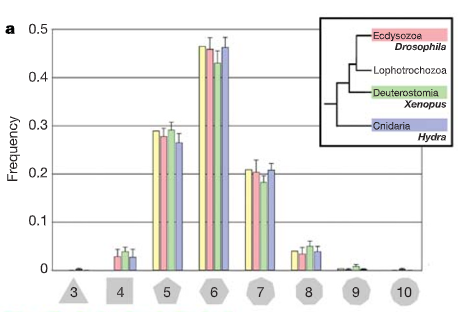
\includegraphics[width=.47\textwidth]{presentation/figures/polygon_distribution_metazoa.png}  
     \caption{Distribution of the predicted and observed polygons (yellow: predicted equilibirum)}
   \end{figure} 
\end{frame}

\begin{frame}[fragile]{Robust equilibrium topology}
  \begin{columns}[onlytextwidth]
    \column{.5\textwidth}
    \begin{figure}
      \centering
      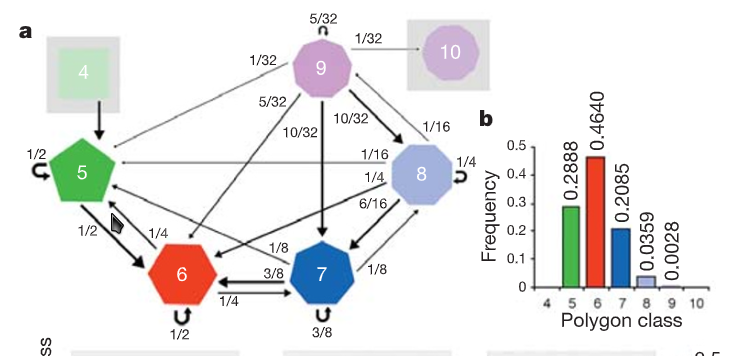
\includegraphics[width=\textwidth]{presentation/figures/fig2a.png}
      \caption{Discrete state dynamics}
    \end{figure}
    \column{.5\textwidth}
    \begin{figure}
      \centering
      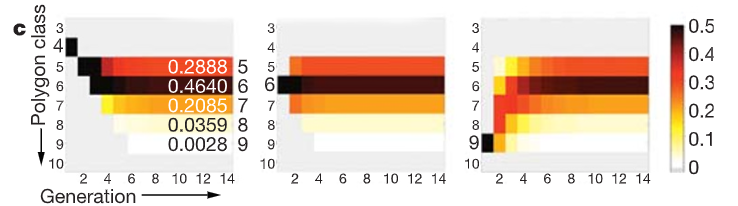
\includegraphics[width=\textwidth]{presentation/figures/fig2c.png}
      \caption{Figure showing the same attained equilibirum, no matter the initial conditions}
    \end{figure}
  \end{columns}  
\end{frame}

\begin{frame}[fragile]{Additional insights on mitotic cells}
  \begin{columns}[onlytextwidth]
    \column{0.45\textwidth}
    As seen in $S$, a mitotic cell gains on average one side, and daughter cells have one less side. Experimental evidence confirms this:
    \begin{table}
      \begin{tabular}{ll}
        \toprule
        \textbf{Non-mitotic cells} & ($5.94\pm 0.06$) \\
        \textbf{Mitotic cells} & ($6.99\pm 0.07$) \\
        \bottomrule 
      \end{tabular}
    \end{table}
    \column{0.5\textwidth}
    \begin{figure}
      \centering
      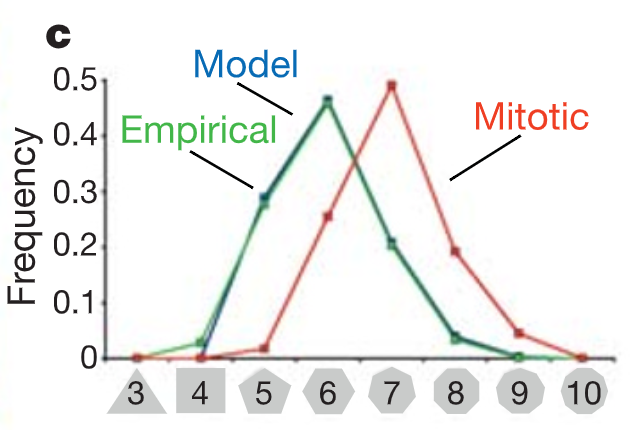
\includegraphics[width=\textwidth]{presentation/figures/fig3c.png}
      \caption{Polygon distributions of mitotic cells vs. non-mitotic cells}
      \label{}
    \end{figure}
  \end{columns}
  $\rightarrow$ cells accumulate sides until division.
\end{frame}

\begin{frame}[fragile]{Polygon distribution of mitotic cells in non-proliferating tissues}
  \begin{columns}[onlytextwidth]
    \column{0.45\textwidth}
    \begin{itemize}
        \item The model does not apply to non-proliferating tissue
        \item Forcing mitosis using \textit{string (stg)} in tissues does not replicate the proliferating tissue distribution.
    \end{itemize}
    \column{0.5\textwidth}
    \begin{figure}
      \centering
      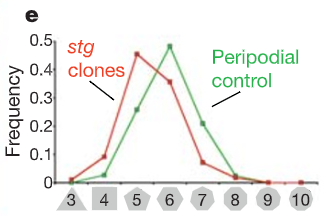
\includegraphics[width=\textwidth]{presentation/figures/fig3e.png}
      \caption{Distribution of polygons in non-proliferating tissue}
    \end{figure}
  \end{columns}
  $\rightarrow$ Differential proliferation influences cell shape and morphogenesis.
\end{frame}

\section{Subsequent works}

\begin{frame}[fragile]{Subsequent work}
  \begin{columns}[T,onlytextwidth]
    \column{0.5\textwidth}
    Work on 3D structures
    \begin{figure}
      \centering
      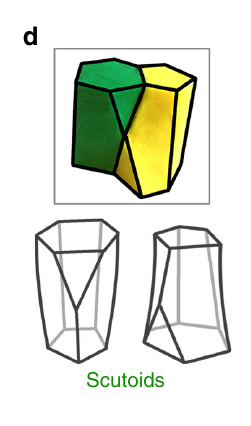
\includegraphics[width=.3\textwidth]{presentation/figures/scutoids.png}
      \caption{The scutoid has been discovered as a solution to 3D cell packing.\cite{gomez2018scutoids}}
    \end{figure}
    \column{.5\textwidth}
    Work on dynamics
    \begin{figure}
      \centering
      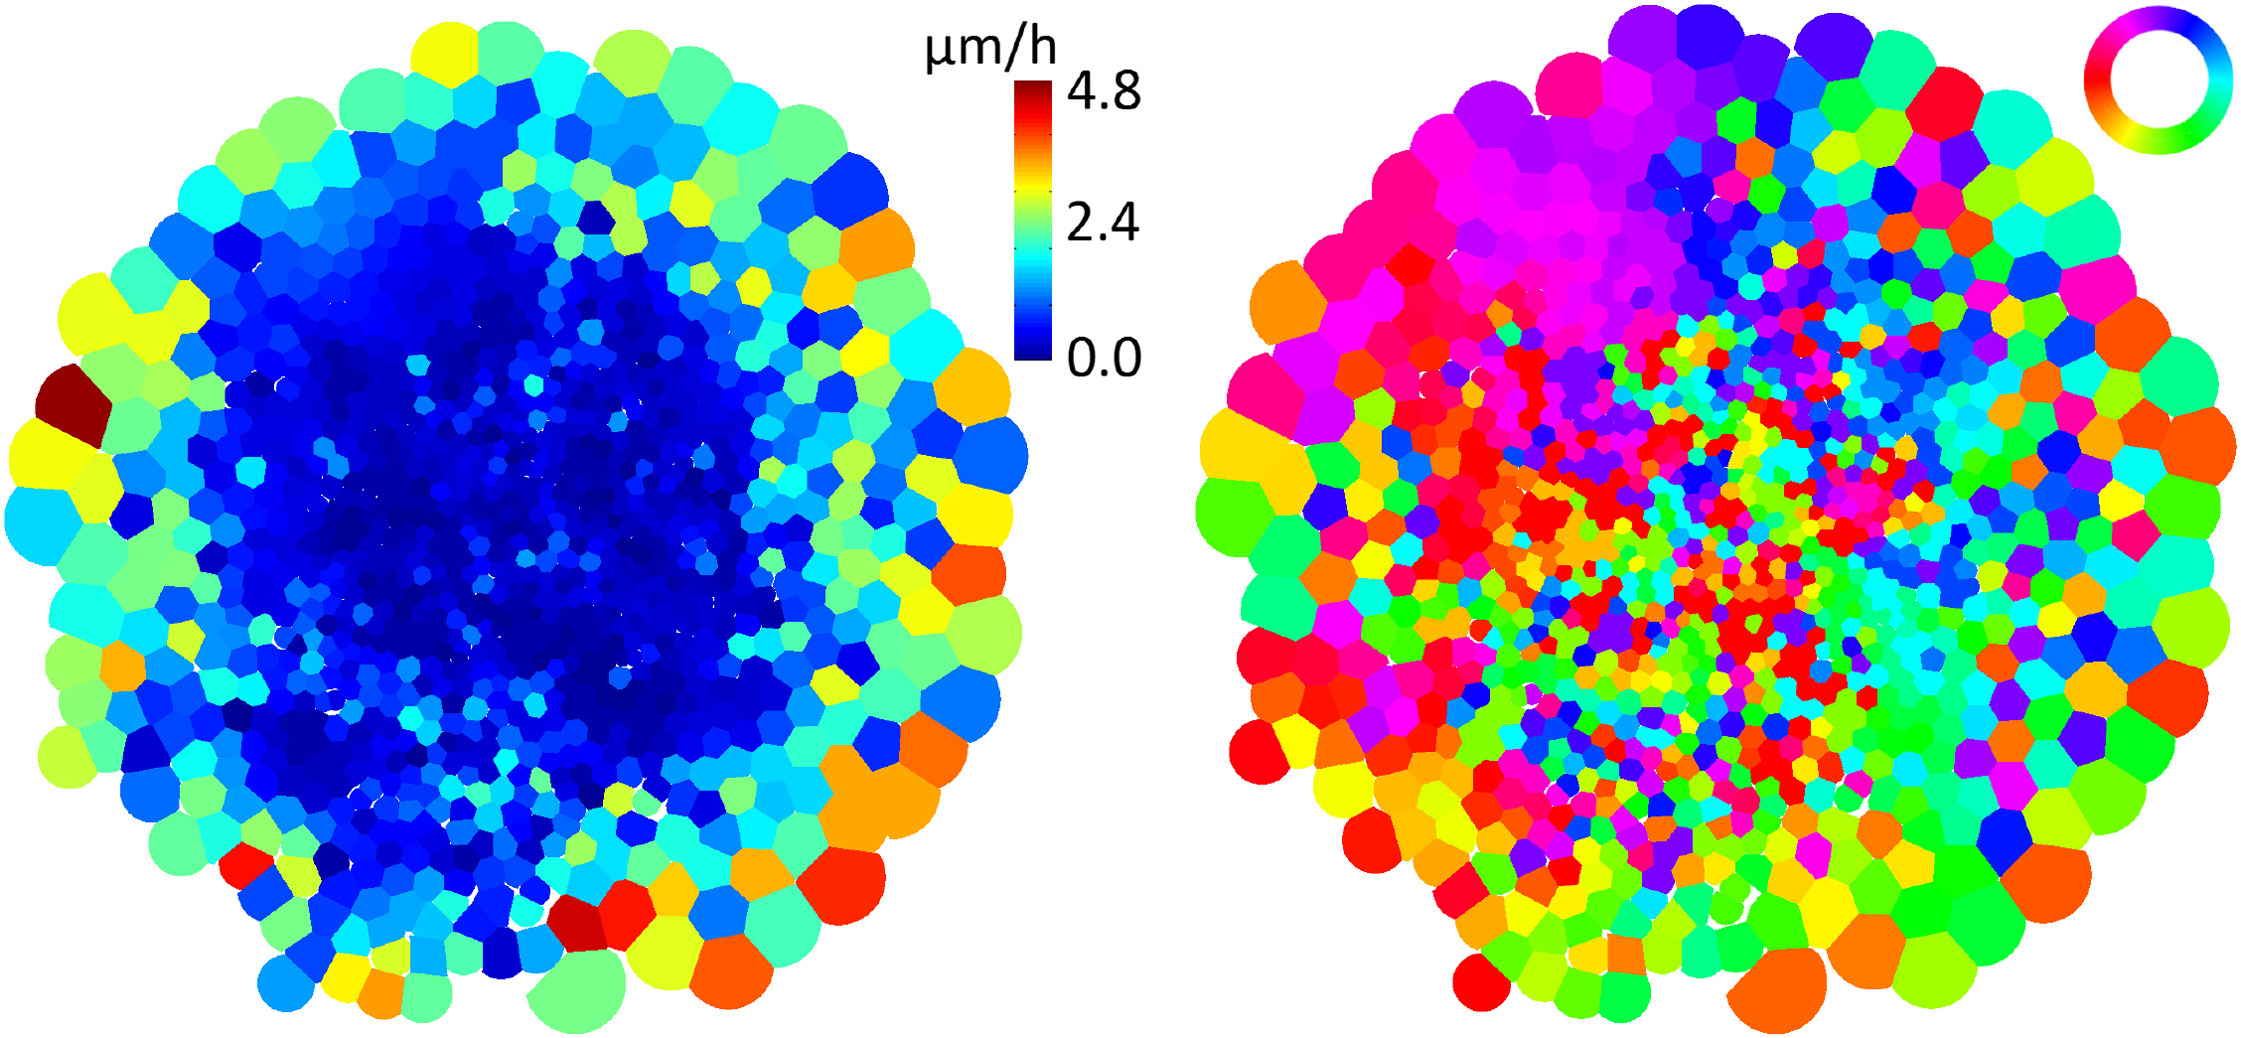
\includegraphics[width=\textwidth]{presentation/figures/Cell_Dynamics.jpg}
      \caption{Modelling and prediction of speed and direction of proliferating epithelia. \cite{aland2015mechanistic}}
      \label{}
    \end{figure}
  \end{columns}
\end{frame}

\section{Conclusions}

\begin{frame}[fragile]{Take home messages} 
  The proposed \textbf{discrete Markov chain}:
  \begin{enumerate}
    \item shows how epithelial topology can be irregular, but \textbf{not random}.
    \onslide<2->\item \textbf{explains the predominantly hexagonal topology} of growing epithelia as well as the distribution of other polygons.
    \onslide<3->\item shows an \textbf{emergent mechanism} by which epithelia accomodate \textbf{rapid proliferation} while maintaining \textbf{structural integrity}.
  \end{enumerate}
\end{frame}

\begin{frame}[standout]
  Questions?
  \vspace{3cm}
  \begin{center}{\Large \faicon{github}} \normalsize\url{https://github.com/pjhartout/CBB_Seminar}\end{center}
\end{frame}

\appendix

\begin{frame}[fragile]{Geometry of \emph{growing} epithelial cells}    
    
  \begin{columns}[onlytextwidth]
      \column{0.5\textwidth}
      Time-lapse movies collected revealed the following findings:
        \begin{itemize}
          \item Initially polygonal prophase cells rounded up and divided
          \item Cell-neighbour relationships were stably maintained throughout the cell cycle
          \item The topology of the divided cells is invariant over time.
        \end{itemize}
     
       
      \column{0.5\textwidth}
          \begin{figure}
              \centering
              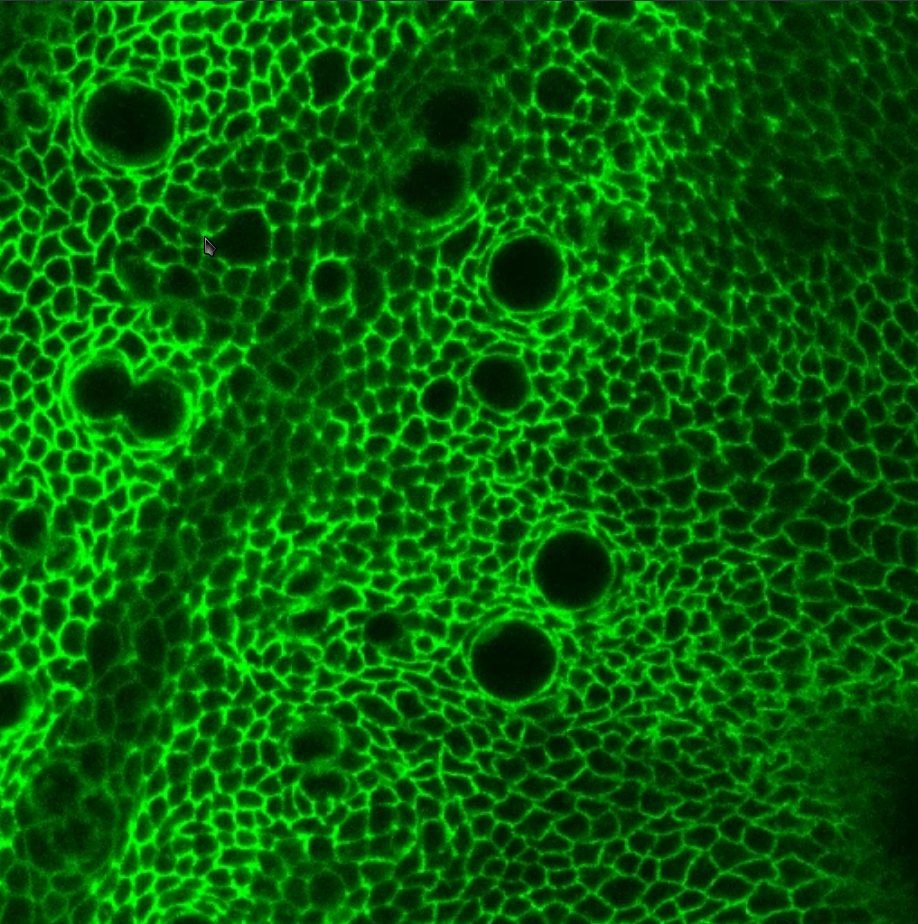
\includegraphics[width=.7\textwidth]{presentation/figures/supfig1.png}
              \caption{General hexagon-dominated topology of growing epithelial in \emph{Drosophila Melanogaster}.}
              \label{}
          \end{figure}
  \end{columns}
\end{frame}


\begin{frame}[fragile]{Derivation of Markov state dynamics - transition matrix $P$}
  \centering
  \begin{columns}[onlytextwidth]
    \column{0.5\textwidth}
    \begin{itemize}
      \item $P_{ij}$: the probabilty that an $i$ sided cell divides to produce a $j$-sided daughter cell.
      \item $K_t$: the number of junctions distributed to one daughter cell on division at generation $t$. $s_{t-1}-K_t$ are left for the other.
      \onslide<2->\item Because no triangular cells are observed, each daughter receives at least two junctions, leaving $s_t-4$ junctions to be distributed among the daughters with equal probability.
      \item So, the number of junctions received by the first daughter is $K_t-2\sim\mathcal{B}(n=s_{t-1}, p=\frac{1}{2})$. 
    \end{itemize}
    \column{0.5\textwidth}
    \begin{itemize}
      \onslide<3->\item As a result $P_{ij}=P(K_t+2=j|s_{t-1}=i)={i-4 \choose j-4}\cdot\frac{1}{2^{i-4}}$
      \onslide<4->\item Therefore, the unnormalized entries of $P$ are the coefficients of Pascal's triangle:
      \renewcommand{\kbldelim}{(}% Left delimiter
      \renewcommand{\kbrdelim}{)}% Right delimiter
      \[
        P = \kbordermatrix{
          & 4 & 5 & 6 & 7 & 8 & 9 & \ldots\\
          4 & 1 &  &  &  & & &  \\
          5 & 1 & 1 & & & & &\\
          6 & 1 & 2 & 1 & & & &\\
          7 & 1 & 3 & 3 & 1 & & & \\
          8 & 1 & 4 & 6 & 4 & 1 & &\\
          9 & 1 & 5 & 10 & 10 & 5 & 1 & \\
          \vdots & & & & & & & \ddots\\
        }
      \]
    \end{itemize}
  \end{columns}
\end{frame}


\begin{frame}[fragile]{Derivation of Markov state dynamics - transition matrix $S$}
  \centering
  \begin{columns}[T,onlytextwidth]
    \column{0.5\textwidth}
    \begin{itemize}
      \item $S_{ij}$: the probability of an $i$-sided cell will gain sides from dividing neighbour cells divisions\\
      \onslide<2-> \item On mitosis, a cell adds one side to each of two neighbouring cells. 
      \onslide<3-> \item Assuming $N$ cells in an epithelium, the number of cells after one round of divisions is $2N$ 
      \onslide<4->\item On average the number of sides gained per cell is $\frac{2N}{2N}=1$. That is, a cell will gain 1 side every cycle on average.
      \onslide<5->\item Thus, $S_{ij}=1$ if $j=i+1$ and 0 otherwise.
    \end{itemize}
    \column{0.5\textwidth} 
      \renewcommand{\kbldelim}{(}% Left delimiter
      \renewcommand{\kbrdelim}{)}% Right delimiter
      \[
        S = \kbordermatrix{
          & 4 & 5 & 6 & 7 & 8 & 9 & \ldots\\
          4 & 0 & 1 &  &  & & &  \\
          5 & & 0 & 1 & & & &\\
          6 & & & 0 & 1 & & &\\
          7 & & & & 0 & 1 & & \\
          8 & & & & & 0 & 1 &\\
          9 & & & & & & 0 & 1\\
          \vdots & & & & & & & \ddots\\
        }
      \]    
  \end{columns}
\end{frame}

\begin{frame}[fragile]{Backup slides - Assumptions of the recurrence system}
  From the aforementioned observations observations we make the following assumptions about the mathematical modelling of cell epithelia: 
  \begin{itemize}
    \item Cells are polygons with a minimum of four sides
    \item Cells do not resort
    \item Mitotic siblings retain a common common junctional interface
    \item Cells have asynchronous but uniform cell cycle times
    \item Cleavage places cut a side rather than a vertex of the mother polygon
    \item Mitotic cleavage orientation randomly distributes existing tricellular junctions to both daughter cells.
  \end{itemize} 
\end{frame}

\begin{frame}[fragile]{Recurrence system}
  \begin{columns}
  \column{0.6\textwidth}  
  \begin{table}
    \caption{Cell features, topological equivalence and evolution at division $t$}
    \scalebox{0.9}{
    \begin{tabular}{lll}
      \toprule
      Cell feature & Graph equivalent & Evolution at division $t$\\
      \midrule
      Tricellular junction & Vertex, $v_t$ & $v_t=v_{t-1}+2f_t$\\ 
      Cell side & Edge, $e_t$ & $e_t=e_{t-1}+3f_{t-1}$\\
      Apical cell surface & Face, $f_t$ & $e_t=e_{t-1}+3f_{t-1}$\\
      \bottomrule
    \end{tabular}
    } 
  \end{table}
  \column{0.4\textwidth}
  So we can construct the following system: 
  \begin{equation*}
    s_t=\frac{2(e_t+3f_{t-1})}{2f_{t-1}}=\frac{s_{t-1}}{2}+3
  \end{equation*}
  which exponentially converges to 6 provided the initial condition:
  \begin{equation*}
    s_t=6+2^{-t}(s_0-6)
  \end{equation*} 
\end{columns}
\end{frame}

\begin{frame}[allowframebreaks]{References}
  
  \bibliographystyle{unsrt}
  \bibliography{References}

\end{frame}


\end{document}